\documentclass[1p]{elsarticle_modified}
%\bibliographystyle{elsarticle-num}

%\usepackage[colorlinks]{hyperref}
%\usepackage{abbrmath_seonhwa} %\Abb, \Ascr, \Acal ,\Abf, \Afrak
\usepackage{amsfonts}
\usepackage{amssymb}
\usepackage{amsmath}
\usepackage{amsthm}
\usepackage{scalefnt}
\usepackage{amsbsy}
\usepackage{kotex}
\usepackage{caption}
\usepackage{subfig}
\usepackage{color}
\usepackage{graphicx}
\usepackage{xcolor} %% white, black, red, green, blue, cyan, magenta, yellow
\usepackage{float}
\usepackage{setspace}
\usepackage{hyperref}

\usepackage{tikz}
\usetikzlibrary{arrows}

\usepackage{multirow}
\usepackage{array} % fixed length table
\usepackage{hhline}

%%%%%%%%%%%%%%%%%%%%%
\makeatletter
\renewcommand*\env@matrix[1][\arraystretch]{%
	\edef\arraystretch{#1}%
	\hskip -\arraycolsep
	\let\@ifnextchar\new@ifnextchar
	\array{*\c@MaxMatrixCols c}}
\makeatother %https://tex.stackexchange.com/questions/14071/how-can-i-increase-the-line-spacing-in-a-matrix
%%%%%%%%%%%%%%%

\usepackage[normalem]{ulem}

\newcommand{\msout}[1]{\ifmmode\text{\sout{\ensuremath{#1}}}\else\sout{#1}\fi}
%SOURCE: \msout is \stkout macro in https://tex.stackexchange.com/questions/20609/strikeout-in-math-mode

\newcommand{\cancel}[1]{
	\ifmmode
	{\color{red}\msout{#1}}
	\else
	{\color{red}\sout{#1}}
	\fi
}

\newcommand{\add}[1]{
	{\color{blue}\uwave{#1}}
}

\newcommand{\replace}[2]{
	\ifmmode
	{\color{red}\msout{#1}}{\color{blue}\uwave{#2}}
	\else
	{\color{red}\sout{#1}}{\color{blue}\uwave{#2}}
	\fi
}

\newcommand{\Sol}{\mathcal{S}} %segment
\newcommand{\D}{D} %diagram
\newcommand{\A}{\mathcal{A}} %arc


%%%%%%%%%%%%%%%%%%%%%%%%%%%%%5 test

\def\sl{\operatorname{\textup{SL}}(2,\Cbb)}
\def\psl{\operatorname{\textup{PSL}}(2,\Cbb)}
\def\quan{\mkern 1mu \triangleright \mkern 1mu}

\theoremstyle{definition}
\newtheorem{thm}{Theorem}[section]
\newtheorem{prop}[thm]{Proposition}
\newtheorem{lem}[thm]{Lemma}
\newtheorem{ques}[thm]{Question}
\newtheorem{cor}[thm]{Corollary}
\newtheorem{defn}[thm]{Definition}
\newtheorem{exam}[thm]{Example}
\newtheorem{rmk}[thm]{Remark}
\newtheorem{alg}[thm]{Algorithm}

\newcommand{\I}{\sqrt{-1}}
\begin{document}

%\begin{frontmatter}
%
%\title{Boundary parabolic representations of knots up to 8 crossings}
%
%%% Group authors per affiliation:
%\author{Yunhi Cho} 
%\address{Department of Mathematics, University of Seoul, Seoul, Korea}
%\ead{yhcho@uos.ac.kr}
%
%
%\author{Seonhwa Kim} %\fnref{s_kim}}
%\address{Center for Geometry and Physics, Institute for Basic Science, Pohang, 37673, Korea}
%\ead{ryeona17@ibs.re.kr}
%
%\author{Hyuk Kim}
%\address{Department of Mathematical Sciences, Seoul National University, Seoul 08826, Korea}
%\ead{hyukkim@snu.ac.kr}
%
%\author{Seokbeom Yoon}
%\address{Department of Mathematical Sciences, Seoul National University, Seoul, 08826,  Korea}
%\ead{sbyoon15@snu.ac.kr}
%
%\begin{abstract}
%We find all boundary parabolic representation of knots up to 8 crossings.
%
%\end{abstract}
%\begin{keyword}
%    \MSC[2010] 57M25 
%\end{keyword}
%
%\end{frontmatter}

%\linenumbers
%\tableofcontents
%
\newcommand\colored[1]{\textcolor{white}{\rule[-0.35ex]{0.8em}{1.4ex}}\kern-0.8em\color{red} #1}%
%\newcommand\colored[1]{\textcolor{white}{ #1}\kern-2.17ex	\textcolor{white}{ #1}\kern-1.81ex	\textcolor{white}{ #1}\kern-2.15ex\color{red}#1	}

{\Large $\underline{12a_{0406}~(K12a_{0406})}$}

\setlength{\tabcolsep}{10pt}
\renewcommand{\arraystretch}{1.6}
\vspace{1cm}\begin{tabular}{m{100pt}>{\centering\arraybackslash}m{274pt}}
\multirow{5}{120pt}{
	\centering
	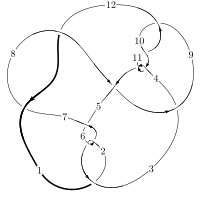
\includegraphics[width=112pt]{../../../GIT/diagram.site/Diagrams/png/1207_12a_0406.png}\\
\ \ \ A knot diagram\footnotemark}&
\allowdisplaybreaks
\textbf{Linearized knot diagam} \\
\cline{2-2}
 &
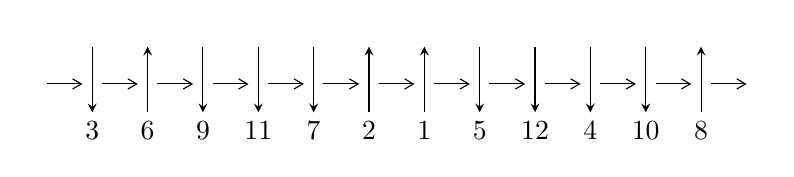
\begin{tikzpicture}[x=20pt, y=17pt]
	% nodes
	\node (C0) at (0, 0) {};
	\node (C1) at (1, 0) {};
	\node (C1U) at (1, +1) {};
	\node (C1D) at (1, -1) {3};

	\node (C2) at (2, 0) {};
	\node (C2U) at (2, +1) {};
	\node (C2D) at (2, -1) {6};

	\node (C3) at (3, 0) {};
	\node (C3U) at (3, +1) {};
	\node (C3D) at (3, -1) {9};

	\node (C4) at (4, 0) {};
	\node (C4U) at (4, +1) {};
	\node (C4D) at (4, -1) {11};

	\node (C5) at (5, 0) {};
	\node (C5U) at (5, +1) {};
	\node (C5D) at (5, -1) {7};

	\node (C6) at (6, 0) {};
	\node (C6U) at (6, +1) {};
	\node (C6D) at (6, -1) {2};

	\node (C7) at (7, 0) {};
	\node (C7U) at (7, +1) {};
	\node (C7D) at (7, -1) {1};

	\node (C8) at (8, 0) {};
	\node (C8U) at (8, +1) {};
	\node (C8D) at (8, -1) {5};

	\node (C9) at (9, 0) {};
	\node (C9U) at (9, +1) {};
	\node (C9D) at (9, -1) {12};

	\node (C10) at (10, 0) {};
	\node (C10U) at (10, +1) {};
	\node (C10D) at (10, -1) {4};

	\node (C11) at (11, 0) {};
	\node (C11U) at (11, +1) {};
	\node (C11D) at (11, -1) {10};

	\node (C12) at (12, 0) {};
	\node (C12U) at (12, +1) {};
	\node (C12D) at (12, -1) {8};
	\node (C13) at (13, 0) {};

	% arrows
	\draw[->,>={angle 60}]
	(C0) edge (C1) (C1) edge (C2) (C2) edge (C3) (C3) edge (C4) (C4) edge (C5) (C5) edge (C6) (C6) edge (C7) (C7) edge (C8) (C8) edge (C9) (C9) edge (C10) (C10) edge (C11) (C11) edge (C12) (C12) edge (C13) ;	\draw[->,>=stealth]
	(C1U) edge (C1D) (C2D) edge (C2U) (C3U) edge (C3D) (C4U) edge (C4D) (C5U) edge (C5D) (C6D) edge (C6U) (C7D) edge (C7U) (C8U) edge (C8D) (C9U) edge (C9D) (C10U) edge (C10D) (C11U) edge (C11D) (C12D) edge (C12U) ;
	\end{tikzpicture} \\
\hhline{~~} \\& 
\textbf{Solving Sequence} \\ \cline{2-2} 
 &
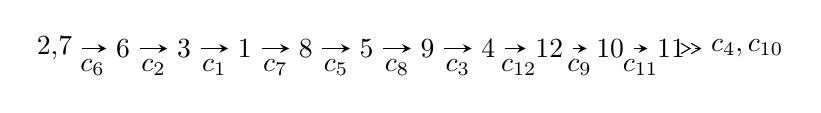
\begin{tikzpicture}[x=22pt, y=7pt]
	% node
	\node (A0) at (-1/8, 0) {2,7};
	\node (A1) at (1, 0) {6};
	\node (A2) at (2, 0) {3};
	\node (A3) at (3, 0) {1};
	\node (A4) at (4, 0) {8};
	\node (A5) at (5, 0) {5};
	\node (A6) at (6, 0) {9};
	\node (A7) at (7, 0) {4};
	\node (A8) at (8, 0) {12};
	\node (A9) at (9, 0) {10};
	\node (A10) at (10, 0) {11};
	\node (C1) at (1/2, -1) {$c_{6}$};
	\node (C2) at (3/2, -1) {$c_{2}$};
	\node (C3) at (5/2, -1) {$c_{1}$};
	\node (C4) at (7/2, -1) {$c_{7}$};
	\node (C5) at (9/2, -1) {$c_{5}$};
	\node (C6) at (11/2, -1) {$c_{8}$};
	\node (C7) at (13/2, -1) {$c_{3}$};
	\node (C8) at (15/2, -1) {$c_{12}$};
	\node (C9) at (17/2, -1) {$c_{9}$};
	\node (C10) at (19/2, -1) {$c_{11}$};
	\node (A11) at (45/4, 0) {$c_{4},c_{10}$};

	% edge
	\draw[->,>=stealth]	
	(A0) edge (A1) (A1) edge (A2) (A2) edge (A3) (A3) edge (A4) (A4) edge (A5) (A5) edge (A6) (A6) edge (A7) (A7) edge (A8) (A8) edge (A9) (A9) edge (A10) ;
	\draw[->>,>={angle 60}]	
	(A10) edge (A11);
\end{tikzpicture} \\ 

\end{tabular} \\

\footnotetext{
The image of knot diagram is generated by the software ``\textbf{Draw programme}" developed by Andrew Bartholomew(\url{http://www.layer8.co.uk/maths/draw/index.htm\#Running-draw}), where we modified some parts for our purpose(\url{https://github.com/CATsTAILs/LinksPainter}).
}\phantom \\ \newline 
\centering \textbf{Ideals for irreducible components\footnotemark of $X_{\text{par}}$} 
 
\begin{align*}
I^u_{1}&=\langle 
u^{89}+u^{88}+\cdots+u-1\rangle \\
\\
\end{align*}
\raggedright * 1 irreducible components of $\dim_{\mathbb{C}}=0$, with total 89 representations.\\
\footnotetext{All coefficients of polynomials are rational numbers. But the coefficients are sometimes approximated in decimal forms when there is not enough margin.}
\newpage
\renewcommand{\arraystretch}{1}
\centering \section*{I. $I^u_{1}= \langle u^{89}+u^{88}+\cdots+u-1 \rangle$}
\flushleft \textbf{(i) Arc colorings}\\
\begin{tabular}{m{7pt} m{180pt} m{7pt} m{180pt} }
\flushright $a_{2}=$&$\begin{pmatrix}0\\u\end{pmatrix}$ \\
\flushright $a_{7}=$&$\begin{pmatrix}1\\0\end{pmatrix}$ \\
\flushright $a_{6}=$&$\begin{pmatrix}1\\u^2\end{pmatrix}$ \\
\flushright $a_{3}=$&$\begin{pmatrix}u\\u^3+u\end{pmatrix}$ \\
\flushright $a_{1}=$&$\begin{pmatrix}u^3\\u^5+u^3+u\end{pmatrix}$ \\
\flushright $a_{8}=$&$\begin{pmatrix}- u^8- u^6- u^4+1\\- u^{10}-2 u^8-3 u^6-2 u^4- u^2\end{pmatrix}$ \\
\flushright $a_{5}=$&$\begin{pmatrix}u^2+1\\u^2\end{pmatrix}$ \\
\flushright $a_{9}=$&$\begin{pmatrix}u^{14}+3 u^{12}+6 u^{10}+7 u^8+6 u^6+4 u^4+2 u^2+1\\u^{14}+2 u^{12}+3 u^{10}+2 u^8- u^2\end{pmatrix}$ \\
\flushright $a_{4}=$&$\begin{pmatrix}- u^{31}-6 u^{29}+\cdots-18 u^5-6 u^3\\- u^{31}-5 u^{29}+\cdots+2 u^3+u\end{pmatrix}$ \\
\flushright $a_{12}=$&$\begin{pmatrix}u^{13}+2 u^{11}+3 u^9+2 u^7- u\\u^{15}+3 u^{13}+6 u^{11}+7 u^9+6 u^7+4 u^5+2 u^3+u\end{pmatrix}$ \\
\flushright $a_{10}=$&$\begin{pmatrix}u^{42}+7 u^{40}+\cdots+u^2+1\\u^{44}+8 u^{42}+\cdots+22 u^6+5 u^4\end{pmatrix}$ \\
\flushright $a_{11}=$&$\begin{pmatrix}u^{71}+12 u^{69}+\cdots+16 u^5+4 u^3\\u^{73}+13 u^{71}+\cdots+2 u^3+u\end{pmatrix}$\\&\end{tabular}
\flushleft \textbf{(ii) Obstruction class $= -1$}\\~\\
\flushleft \textbf{(iii) Cusp Shapes $= -4 u^{88}-60 u^{86}+\cdots+16 u-10$}\\~\\
\newpage\renewcommand{\arraystretch}{1}
\flushleft \textbf{(iv) u-Polynomials at the component}\newline \\
\begin{tabular}{m{50pt}|m{274pt}}
Crossings & \hspace{64pt}u-Polynomials at each crossing \\
\hline $$\begin{aligned}c_{1},c_{5}\end{aligned}$$&$\begin{aligned}
&u^{89}+31 u^{88}+\cdots-3 u-1
\end{aligned}$\\
\hline $$\begin{aligned}c_{2},c_{6}\end{aligned}$$&$\begin{aligned}
&u^{89}- u^{88}+\cdots+u+1
\end{aligned}$\\
\hline $$\begin{aligned}c_{3}\end{aligned}$$&$\begin{aligned}
&u^{89}+u^{88}+\cdots+361 u+97
\end{aligned}$\\
\hline $$\begin{aligned}c_{4},c_{10}\end{aligned}$$&$\begin{aligned}
&u^{89}- u^{88}+\cdots+u+1
\end{aligned}$\\
\hline $$\begin{aligned}c_{7},c_{12}\end{aligned}$$&$\begin{aligned}
&u^{89}+5 u^{88}+\cdots+107 u+21
\end{aligned}$\\
\hline $$\begin{aligned}c_{8}\end{aligned}$$&$\begin{aligned}
&u^{89}-7 u^{88}+\cdots-1205 u-391
\end{aligned}$\\
\hline $$\begin{aligned}c_{9},c_{11}\end{aligned}$$&$\begin{aligned}
&u^{89}+29 u^{88}+\cdots-3 u+1
\end{aligned}$\\
\hline
\end{tabular}\\~\\
\newpage\renewcommand{\arraystretch}{1}
\flushleft \textbf{(v) Riley Polynomials at the component}\newline \\
\begin{tabular}{m{50pt}|m{274pt}}
Crossings & \hspace{64pt}Riley Polynomials at each crossing \\
\hline $$\begin{aligned}c_{1},c_{5}\end{aligned}$$&$\begin{aligned}
&y^{89}+55 y^{88}+\cdots+5 y-1
\end{aligned}$\\
\hline $$\begin{aligned}c_{2},c_{6}\end{aligned}$$&$\begin{aligned}
&y^{89}+31 y^{88}+\cdots-3 y-1
\end{aligned}$\\
\hline $$\begin{aligned}c_{3}\end{aligned}$$&$\begin{aligned}
&y^{89}-9 y^{88}+\cdots+469821 y-9409
\end{aligned}$\\
\hline $$\begin{aligned}c_{4},c_{10}\end{aligned}$$&$\begin{aligned}
&y^{89}-29 y^{88}+\cdots-3 y-1
\end{aligned}$\\
\hline $$\begin{aligned}c_{7},c_{12}\end{aligned}$$&$\begin{aligned}
&y^{89}+59 y^{88}+\cdots-9131 y-441
\end{aligned}$\\
\hline $$\begin{aligned}c_{8}\end{aligned}$$&$\begin{aligned}
&y^{89}+11 y^{88}+\cdots-5202795 y-152881
\end{aligned}$\\
\hline $$\begin{aligned}c_{9},c_{11}\end{aligned}$$&$\begin{aligned}
&y^{89}+63 y^{88}+\cdots-27 y-1
\end{aligned}$\\
\hline
\end{tabular}\\~\\
\newpage\flushleft \textbf{(vi) Complex Volumes and Cusp Shapes}
$$\begin{array}{c|c|c}  
\text{Solutions to }I^u_{1}& \I (\text{vol} + \sqrt{-1}CS) & \text{Cusp shape}\\
 \hline 
\begin{aligned}
u &= \phantom{-}0.792424 + 0.618504 I\end{aligned}
 & \phantom{-}3.11119 - 5.13284 I & \phantom{-0.000000 } 0 \\ \hline\begin{aligned}
u &= \phantom{-}0.792424 - 0.618504 I\end{aligned}
 & \phantom{-}3.11119 + 5.13284 I & \phantom{-0.000000 } 0 \\ \hline\begin{aligned}
u &= -0.796751 + 0.614079 I\end{aligned}
 & \phantom{-}2.10885 + 10.87920 I & \phantom{-0.000000 } 0 \\ \hline\begin{aligned}
u &= -0.796751 - 0.614079 I\end{aligned}
 & \phantom{-}2.10885 - 10.87920 I & \phantom{-0.000000 } 0 \\ \hline\begin{aligned}
u &= \phantom{-}0.756551 + 0.674024 I\end{aligned}
 & \phantom{-}5.26973 - 2.66595 I & \phantom{-0.000000 } 0 \\ \hline\begin{aligned}
u &= \phantom{-}0.756551 - 0.674024 I\end{aligned}
 & \phantom{-}5.26973 + 2.66595 I & \phantom{-0.000000 } 0 \\ \hline\begin{aligned}
u &= -0.781291 + 0.601828 I\end{aligned}
 & -3.26113 + 5.11902 I & \phantom{-0.000000 } 0 \\ \hline\begin{aligned}
u &= -0.781291 - 0.601828 I\end{aligned}
 & -3.26113 - 5.11902 I & \phantom{-0.000000 } 0 \\ \hline\begin{aligned}
u &= -0.749471 + 0.687801 I\end{aligned}
 & \phantom{-}4.91888 - 3.02362 I & \phantom{-0.000000 } 0 \\ \hline\begin{aligned}
u &= -0.749471 - 0.687801 I\end{aligned}
 & \phantom{-}4.91888 + 3.02362 I & \phantom{-0.000000 } 0 \\ \hline\begin{aligned}
u &= \phantom{-}0.762514 + 0.617485 I\end{aligned}
 & \phantom{-}0.72677 - 2.95488 I & \phantom{-0.000000 } 0 \\ \hline\begin{aligned}
u &= \phantom{-}0.762514 - 0.617485 I\end{aligned}
 & \phantom{-}0.72677 + 2.95488 I & \phantom{-0.000000 } 0 \\ \hline\begin{aligned}
u &= -0.050173 + 0.978604 I\end{aligned}
 & -0.29363 - 2.69848 I & \phantom{-0.000000 } 0 \\ \hline\begin{aligned}
u &= -0.050173 - 0.978604 I\end{aligned}
 & -0.29363 + 2.69848 I & \phantom{-0.000000 } 0 \\ \hline\begin{aligned}
u &= \phantom{-}0.414241 + 0.879359 I\end{aligned}
 & \phantom{-}0.79840 + 7.49051 I & \phantom{-0.000000 } 0 \\ \hline\begin{aligned}
u &= \phantom{-}0.414241 - 0.879359 I\end{aligned}
 & \phantom{-}0.79840 - 7.49051 I & \phantom{-0.000000 } 0 \\ \hline\begin{aligned}
u &= -0.448726 + 0.856142 I\end{aligned}
 & \phantom{-}1.61410 - 2.05998 I & \phantom{-0.000000 } 0 \\ \hline\begin{aligned}
u &= -0.448726 - 0.856142 I\end{aligned}
 & \phantom{-}1.61410 + 2.05998 I & \phantom{-0.000000 } 0 \\ \hline\begin{aligned}
u &= -0.746043 + 0.583768 I\end{aligned}
 & -1.104240 - 0.816505 I & \phantom{-0.000000 } 0 \\ \hline\begin{aligned}
u &= -0.746043 - 0.583768 I\end{aligned}
 & -1.104240 + 0.816505 I & \phantom{-0.000000 } 0 \\ \hline\begin{aligned}
u &= -0.705718 + 0.816241 I\end{aligned}
 & \phantom{-}1.374950 - 0.274630 I & \phantom{-0.000000 } 0 \\ \hline\begin{aligned}
u &= -0.705718 - 0.816241 I\end{aligned}
 & \phantom{-}1.374950 + 0.274630 I & \phantom{-0.000000 } 0 \\ \hline\begin{aligned}
u &= -0.037143 + 1.080270 I\end{aligned}
 & -5.00271 - 2.21550 I & \phantom{-0.000000 } 0 \\ \hline\begin{aligned}
u &= -0.037143 - 1.080270 I\end{aligned}
 & -5.00271 + 2.21550 I & \phantom{-0.000000 } 0 \\ \hline\begin{aligned}
u &= -0.063504 + 1.094470 I\end{aligned}
 & -2.92880 - 4.38942 I & \phantom{-0.000000 } 0 \\ \hline\begin{aligned}
u &= -0.063504 - 1.094470 I\end{aligned}
 & -2.92880 + 4.38942 I & \phantom{-0.000000 } 0 \\ \hline\begin{aligned}
u &= \phantom{-}0.018621 + 1.097080 I\end{aligned}
 & -6.71736 - 1.83677 I & \phantom{-0.000000 } 0 \\ \hline\begin{aligned}
u &= \phantom{-}0.018621 - 1.097080 I\end{aligned}
 & -6.71736 + 1.83677 I & \phantom{-0.000000 } 0 \\ \hline\begin{aligned}
u &= \phantom{-}0.045471 + 1.100660 I\end{aligned}
 & -9.16961 + 4.22423 I & \phantom{-0.000000 } 0 \\ \hline\begin{aligned}
u &= \phantom{-}0.045471 - 1.100660 I\end{aligned}
 & -9.16961 - 4.22423 I & \phantom{-0.000000 } 0\\
 \hline 
 \end{array}$$\newpage$$\begin{array}{c|c|c}  
\text{Solutions to }I^u_{1}& \I (\text{vol} + \sqrt{-1}CS) & \text{Cusp shape}\\
 \hline 
\begin{aligned}
u &= \phantom{-}0.063947 + 1.101120 I\end{aligned}
 & -3.96933 + 10.08100 I & \phantom{-0.000000 } 0 \\ \hline\begin{aligned}
u &= \phantom{-}0.063947 - 1.101120 I\end{aligned}
 & -3.96933 - 10.08100 I & \phantom{-0.000000 } 0 \\ \hline\begin{aligned}
u &= \phantom{-}0.111277 + 0.878977 I\end{aligned}
 & -0.48030 - 2.60995 I & -8.16580 + 1.81655 I \\ \hline\begin{aligned}
u &= \phantom{-}0.111277 - 0.878977 I\end{aligned}
 & -0.48030 + 2.60995 I & -8.16580 - 1.81655 I \\ \hline\begin{aligned}
u &= -0.748159 + 0.826966 I\end{aligned}
 & \phantom{-}6.86792 + 4.32397 I & \phantom{-0.000000 } 0 \\ \hline\begin{aligned}
u &= -0.748159 - 0.826966 I\end{aligned}
 & \phantom{-}6.86792 - 4.32397 I & \phantom{-0.000000 } 0 \\ \hline\begin{aligned}
u &= \phantom{-}0.715743 + 0.859066 I\end{aligned}
 & \phantom{-}4.12520 + 2.73162 I & \phantom{-0.000000 } 0 \\ \hline\begin{aligned}
u &= \phantom{-}0.715743 - 0.859066 I\end{aligned}
 & \phantom{-}4.12520 - 2.73162 I & \phantom{-0.000000 } 0 \\ \hline\begin{aligned}
u &= \phantom{-}0.701524 + 0.532948 I\end{aligned}
 & -1.45390 - 3.14036 I & -5.81541 + 3.08693 I \\ \hline\begin{aligned}
u &= \phantom{-}0.701524 - 0.532948 I\end{aligned}
 & -1.45390 + 3.14036 I & -5.81541 - 3.08693 I \\ \hline\begin{aligned}
u &= \phantom{-}0.745460 + 0.835125 I\end{aligned}
 & \phantom{-}7.56666 + 1.42671 I & \phantom{-0.000000 } 0 \\ \hline\begin{aligned}
u &= \phantom{-}0.745460 - 0.835125 I\end{aligned}
 & \phantom{-}7.56666 - 1.42671 I & \phantom{-0.000000 } 0 \\ \hline\begin{aligned}
u &= \phantom{-}0.313983 + 0.821757 I\end{aligned}
 & -3.73770 + 2.25778 I & -12.76156 - 5.27279 I \\ \hline\begin{aligned}
u &= \phantom{-}0.313983 - 0.821757 I\end{aligned}
 & -3.73770 - 2.25778 I & -12.76156 + 5.27279 I \\ \hline\begin{aligned}
u &= -0.702092 + 0.892182 I\end{aligned}
 & \phantom{-}1.14647 - 5.11858 I & \phantom{-0.000000 } 0 \\ \hline\begin{aligned}
u &= -0.702092 - 0.892182 I\end{aligned}
 & \phantom{-}1.14647 + 5.11858 I & \phantom{-0.000000 } 0 \\ \hline\begin{aligned}
u &= \phantom{-}0.735138 + 0.888062 I\end{aligned}
 & \phantom{-}7.40603 + 4.18505 I & \phantom{-0.000000 } 0 \\ \hline\begin{aligned}
u &= \phantom{-}0.735138 - 0.888062 I\end{aligned}
 & \phantom{-}7.40603 - 4.18505 I & \phantom{-0.000000 } 0 \\ \hline\begin{aligned}
u &= -0.734636 + 0.895406 I\end{aligned}
 & \phantom{-}6.66040 - 9.94218 I & \phantom{-0.000000 } 0 \\ \hline\begin{aligned}
u &= -0.734636 - 0.895406 I\end{aligned}
 & \phantom{-}6.66040 + 9.94218 I & \phantom{-0.000000 } 0 \\ \hline\begin{aligned}
u &= -0.611338 + 0.569358 I\end{aligned}
 & -0.124299 - 0.982347 I & -2.27042 + 3.59861 I \\ \hline\begin{aligned}
u &= -0.611338 - 0.569358 I\end{aligned}
 & -0.124299 + 0.982347 I & -2.27042 - 3.59861 I \\ \hline\begin{aligned}
u &= -0.599043 + 1.012220 I\end{aligned}
 & \phantom{-}0.31919 - 2.05341 I & \phantom{-0.000000 } 0 \\ \hline\begin{aligned}
u &= -0.599043 - 1.012220 I\end{aligned}
 & \phantom{-}0.31919 + 2.05341 I & \phantom{-0.000000 } 0 \\ \hline\begin{aligned}
u &= \phantom{-}0.596824 + 1.020580 I\end{aligned}
 & -0.71708 - 3.53466 I & \phantom{-0.000000 } 0 \\ \hline\begin{aligned}
u &= \phantom{-}0.596824 - 1.020580 I\end{aligned}
 & -0.71708 + 3.53466 I & \phantom{-0.000000 } 0 \\ \hline\begin{aligned}
u &= \phantom{-}0.662757 + 0.464863 I\end{aligned}
 & -4.15479 + 2.64865 I & -8.87639 - 4.03321 I \\ \hline\begin{aligned}
u &= \phantom{-}0.662757 - 0.464863 I\end{aligned}
 & -4.15479 - 2.64865 I & -8.87639 + 4.03321 I \\ \hline\begin{aligned}
u &= -0.632747 + 1.010330 I\end{aligned}
 & -1.35976 - 4.01784 I & \phantom{-0.000000 } 0 \\ \hline\begin{aligned}
u &= -0.632747 - 1.010330 I\end{aligned}
 & -1.35976 + 4.01784 I & \phantom{-0.000000 } 0\\
 \hline 
 \end{array}$$\newpage$$\begin{array}{c|c|c}  
\text{Solutions to }I^u_{1}& \I (\text{vol} + \sqrt{-1}CS) & \text{Cusp shape}\\
 \hline 
\begin{aligned}
u &= \phantom{-}0.616311 + 1.024920 I\end{aligned}
 & -5.65284 + 2.29612 I & \phantom{-0.000000 } 0 \\ \hline\begin{aligned}
u &= \phantom{-}0.616311 - 1.024920 I\end{aligned}
 & -5.65284 - 2.29612 I & \phantom{-0.000000 } 0 \\ \hline\begin{aligned}
u &= -0.687197 + 0.991834 I\end{aligned}
 & \phantom{-}4.00117 - 2.45258 I & \phantom{-0.000000 } 0 \\ \hline\begin{aligned}
u &= -0.687197 - 0.991834 I\end{aligned}
 & \phantom{-}4.00117 + 2.45258 I & \phantom{-0.000000 } 0 \\ \hline\begin{aligned}
u &= \phantom{-}0.638227 + 1.029020 I\end{aligned}
 & -2.85651 + 8.30192 I & \phantom{-0.000000 } 0 \\ \hline\begin{aligned}
u &= \phantom{-}0.638227 - 1.029020 I\end{aligned}
 & -2.85651 - 8.30192 I & \phantom{-0.000000 } 0 \\ \hline\begin{aligned}
u &= \phantom{-}0.688393 + 1.000560 I\end{aligned}
 & \phantom{-}4.28705 + 8.16569 I & \phantom{-0.000000 } 0 \\ \hline\begin{aligned}
u &= \phantom{-}0.688393 - 1.000560 I\end{aligned}
 & \phantom{-}4.28705 - 8.16569 I & \phantom{-0.000000 } 0 \\ \hline\begin{aligned}
u &= -0.664209 + 1.031080 I\end{aligned}
 & -2.41122 - 4.56435 I & \phantom{-0.000000 } 0 \\ \hline\begin{aligned}
u &= -0.664209 - 1.031080 I\end{aligned}
 & -2.41122 + 4.56435 I & \phantom{-0.000000 } 0 \\ \hline\begin{aligned}
u &= \phantom{-}0.657312 + 0.403482 I\end{aligned}
 & \phantom{-}0.89298 + 8.30474 I & -2.77230 - 7.50293 I \\ \hline\begin{aligned}
u &= \phantom{-}0.657312 - 0.403482 I\end{aligned}
 & \phantom{-}0.89298 - 8.30474 I & -2.77230 + 7.50293 I \\ \hline\begin{aligned}
u &= \phantom{-}0.677609 + 1.026170 I\end{aligned}
 & -0.48705 + 8.43111 I & \phantom{-0.000000 } 0 \\ \hline\begin{aligned}
u &= \phantom{-}0.677609 - 1.026170 I\end{aligned}
 & -0.48705 - 8.43111 I & \phantom{-0.000000 } 0 \\ \hline\begin{aligned}
u &= -0.679374 + 1.036700 I\end{aligned}
 & -4.55418 - 10.64520 I & \phantom{-0.000000 } 0 \\ \hline\begin{aligned}
u &= -0.679374 - 1.036700 I\end{aligned}
 & -4.55418 + 10.64520 I & \phantom{-0.000000 } 0 \\ \hline\begin{aligned}
u &= \phantom{-}0.688505 + 1.034580 I\end{aligned}
 & \phantom{-}1.86598 + 10.72270 I & \phantom{-0.000000 } 0 \\ \hline\begin{aligned}
u &= \phantom{-}0.688505 - 1.034580 I\end{aligned}
 & \phantom{-}1.86598 - 10.72270 I & \phantom{-0.000000 } 0 \\ \hline\begin{aligned}
u &= -0.688639 + 1.037620 I\end{aligned}
 & \phantom{-}0.8409 - 16.4799 I & \phantom{-0.000000 } 0 \\ \hline\begin{aligned}
u &= -0.688639 - 1.037620 I\end{aligned}
 & \phantom{-}0.8409 + 16.4799 I & \phantom{-0.000000 } 0 \\ \hline\begin{aligned}
u &= -0.635260 + 0.400865 I\end{aligned}
 & \phantom{-}1.86099 - 2.66579 I & -0.88903 + 2.73641 I \\ \hline\begin{aligned}
u &= -0.635260 - 0.400865 I\end{aligned}
 & \phantom{-}1.86099 + 2.66579 I & -0.88903 - 2.73641 I \\ \hline\begin{aligned}
u &= -0.349167 + 0.527838 I\end{aligned}
 & -0.135235 - 1.066210 I & -2.23468 + 5.96441 I \\ \hline\begin{aligned}
u &= -0.349167 - 0.527838 I\end{aligned}
 & -0.135235 + 1.066210 I & -2.23468 - 5.96441 I \\ \hline\begin{aligned}
u &= -0.501948 + 0.197273 I\end{aligned}
 & \phantom{-}3.26226 - 1.15588 I & \phantom{-}2.07588 + 2.90357 I \\ \hline\begin{aligned}
u &= -0.501948 - 0.197273 I\end{aligned}
 & \phantom{-}3.26226 + 1.15588 I & \phantom{-}2.07588 - 2.90357 I \\ \hline\begin{aligned}
u &= \phantom{-}0.507837 + 0.153612 I\end{aligned}
 & \phantom{-}2.69964 - 4.37412 I & \phantom{-}0.81673 + 3.12761 I \\ \hline\begin{aligned}
u &= \phantom{-}0.507837 - 0.153612 I\end{aligned}
 & \phantom{-}2.69964 + 4.37412 I & \phantom{-}0.81673 - 3.12761 I \\ \hline\begin{aligned}
u &= \phantom{-}0.403915\phantom{ +0.000000I}\end{aligned}
 & -1.63407\phantom{ +0.000000I} & -4.55070\phantom{ +0.000000I}\\
 \hline 
 \end{array}$$\newpage
\newpage\renewcommand{\arraystretch}{1}
\centering \section*{ II. u-Polynomials}
\begin{tabular}{m{50pt}|m{274pt}}
Crossings & \hspace{64pt}u-Polynomials at each crossing \\
\hline $$\begin{aligned}c_{1},c_{5}\end{aligned}$$&$\begin{aligned}
&u^{89}+31 u^{88}+\cdots-3 u-1
\end{aligned}$\\
\hline $$\begin{aligned}c_{2},c_{6}\end{aligned}$$&$\begin{aligned}
&u^{89}- u^{88}+\cdots+u+1
\end{aligned}$\\
\hline $$\begin{aligned}c_{3}\end{aligned}$$&$\begin{aligned}
&u^{89}+u^{88}+\cdots+361 u+97
\end{aligned}$\\
\hline $$\begin{aligned}c_{4},c_{10}\end{aligned}$$&$\begin{aligned}
&u^{89}- u^{88}+\cdots+u+1
\end{aligned}$\\
\hline $$\begin{aligned}c_{7},c_{12}\end{aligned}$$&$\begin{aligned}
&u^{89}+5 u^{88}+\cdots+107 u+21
\end{aligned}$\\
\hline $$\begin{aligned}c_{8}\end{aligned}$$&$\begin{aligned}
&u^{89}-7 u^{88}+\cdots-1205 u-391
\end{aligned}$\\
\hline $$\begin{aligned}c_{9},c_{11}\end{aligned}$$&$\begin{aligned}
&u^{89}+29 u^{88}+\cdots-3 u+1
\end{aligned}$\\
\hline
\end{tabular}\newpage\renewcommand{\arraystretch}{1}
\centering \section*{ III. Riley Polynomials}
\begin{tabular}{m{50pt}|m{274pt}}
Crossings & \hspace{64pt}Riley Polynomials at each crossing \\
\hline $$\begin{aligned}c_{1},c_{5}\end{aligned}$$&$\begin{aligned}
&y^{89}+55 y^{88}+\cdots+5 y-1
\end{aligned}$\\
\hline $$\begin{aligned}c_{2},c_{6}\end{aligned}$$&$\begin{aligned}
&y^{89}+31 y^{88}+\cdots-3 y-1
\end{aligned}$\\
\hline $$\begin{aligned}c_{3}\end{aligned}$$&$\begin{aligned}
&y^{89}-9 y^{88}+\cdots+469821 y-9409
\end{aligned}$\\
\hline $$\begin{aligned}c_{4},c_{10}\end{aligned}$$&$\begin{aligned}
&y^{89}-29 y^{88}+\cdots-3 y-1
\end{aligned}$\\
\hline $$\begin{aligned}c_{7},c_{12}\end{aligned}$$&$\begin{aligned}
&y^{89}+59 y^{88}+\cdots-9131 y-441
\end{aligned}$\\
\hline $$\begin{aligned}c_{8}\end{aligned}$$&$\begin{aligned}
&y^{89}+11 y^{88}+\cdots-5202795 y-152881
\end{aligned}$\\
\hline $$\begin{aligned}c_{9},c_{11}\end{aligned}$$&$\begin{aligned}
&y^{89}+63 y^{88}+\cdots-27 y-1
\end{aligned}$\\
\hline
\end{tabular}
\vskip 2pc
\end{document}